%**
%*  @file  workflow.tex
%*  @brief   DIET User's Manual workflow chapter file
%*  @author   - Abdelkader Amar (Abdelkader.Amar@ens-lyon.fr)
%*            - Raphael Bolze (Raphael.Bolze@ens-lyon.fr)
%*            - Benjamin Isnard (Benjamin.Isnard@ens-lyon.fr)
%*  @section Licence 
%*    |LICENSE|

\chapter{Workflow management in \textsc{\diet}}
\label{ch:workflows}

\section{Overview}

Workflow applications consist of multiple components (tasks) related by
precedence constraints that usually follow the data flow between
them, \ie data files generated by one task are needed to start another
task. Although this is the most common situation, precedence constraints
may exist for other reasons, and be arbitrarily defined by the user.

This kind of application can be modeled as a \DAG (Directed Acyclic Graph) where
each vertex is a task with given input data and service name, and each edge can
either be a data link between two tasks or a basic precedence constraint. The
\diet workflow engine can handle that kind of workflow by assigning 
those tasks to SeDs using one \diet service call. This assignment is
made internally and dynamically when the task is ready to be executed (\ie all predecessors
are done) depending on the service performance properties and on available
resources on the grid.

A specific agent called the \textbf{Master Agent \DAG (\madag)} provides \DAG
workflow scheduling. This agent serves as the entry point to the \diet
Hierarchy for a client that wants to submit a workflow. The language
supported by the \madag is based on XML and described in
the section \ref{sec:dag_desc}.

Because of large amounts of computations and data involved in some workflow
applications, the number of tasks in a \DAG can grow very fast. The need for a
more abstract way of representing a workflow that separates the data instances
from the data flow has led to the definition of a {\it functional workflow
language} called the \textit{Gwendia language}. A complex application can be
defined using this language which provides data operators and control structures
(if/then/else, loops, \etc). To execute the application, the user needs to provide both
the workflow description (see \ref{sec:wf_desc}) and a file describing the
input data set. The \diet workflow engine then instantiates the workflow as one
or several tasks' \DAGS, sent to the \madag agent to be executed in the
\diet platform.

\section{Quick start}

\paragraph{Requirements and compilation}

The workflow supports in \diet needs the following:

\begin{itemize}
\item The Xerces library: the XML handling code is written with Xerces-C++
  using the provided DOM API.
\item The XQilla library: conditions in conditional or looping workflow
  structures are written in XQuery language and parsed using the XQilla
  library.
\item Enable the workflow support when compiling \diet with the
  \texttt{DIET\_USE\_WORKFLOW} flags set (which can be done in a script or
  command line with \texttt{-DDIET\_USE\_WORKFLOW:BOOL=ON}).

  In case \textit{cmake} is not able to locate the installation of the required
  libraries, you have to set:

\begin{itemize}
\item \texttt{XERCES\_DIR} which defines the path to Xerces installation
  directory, \\ with \texttt{-DXERCES\_DIR:PATH=/usr/local/xerces} for example.
\item \texttt{XQILLA\_DIR} which defines the path to XQilla installation
  directory, \\with \texttt{-DXQILLA\_DIR:PATH=/usr/local/xqilla} for example.
\end{itemize}

\begin{remarque}
By activating the workflow module, the \dagda module is also activated.
\end{remarque}
\begin{remarque}
Workflow support is not available on Windows/Cygwin platforms (Windows XP and
Cygwin $<=$ 1.5.25) for \textit{Xerces} 3.0.1 and \textit{XQilla} 2.2.0.
\end{remarque}


Here is an example of a generating command line:

\verb|cmake ${path_to_diet_sources} \|

\verb|      -DOMNIORB4_DIR=/usr/local/omniORB \|

\verb|      -DDIET_USE_WORKFLOW:BOOL=ON \|

\verb|      -DXERCES_DIR=/usr/local/xerces \|

\verb|      -DXQILLA_DIR=/usr/local/xqilla|

\paragraph{}
Workflow support was tested in the following configurations:

\begin{itemize}
\item gcc version 4.0.2 and higher
\item \textit{omniORB} version 4.1.0 and higher
\item \textit{Xerces} 3.0.1, 3.1.1-r1
\item \textit{XQilla} 2.2.0, 2.3.0
\end{itemize}
\end{itemize}

\paragraph{Executing the examples}
\label{sec:wf_examples}

You need to have a running \diet platform with a \madag agent and the needed
services registered -- You can for example launch a single \sed that includes
all the needed services (\eg \texttt{scalar\_server} if the workflow only
performs operations on scalar). You can find details on how to develop a \sed
in Chapter~\ref{ch:server}.

The directory \texttt{src/examples/workflow} includes several code examples of
workflows. For example,
\begin{itemize}
\item you can find a simple \DAG workflow (see Figure~\ref{fig:example1}) in
  the file \texttt{xml/scalar.xml}. You can test it with a command such as the
  following, where \texttt{local\_client.cfg} is the \diet configuration file
  (\texttt{etc/client\_wf.cfg} is provided as an example);

\verb|./generic_client local_client.cfg -dag scalar.xml |

\item you can also find some examples of functional workflows written in the
  Gwendia language (see file \texttt{xml/func\_string.xml}). You can perform
  some tests with commands such as:

  \verb|./generic_client local_client.cfg -wf func_string.xml data.xml |

%You need to have a running \diet platform with the needed services (the
%commands to launch the services are included as comments within the workflow
%XML).
\end{itemize}

\begin{figure}[htbp]
  \centering
  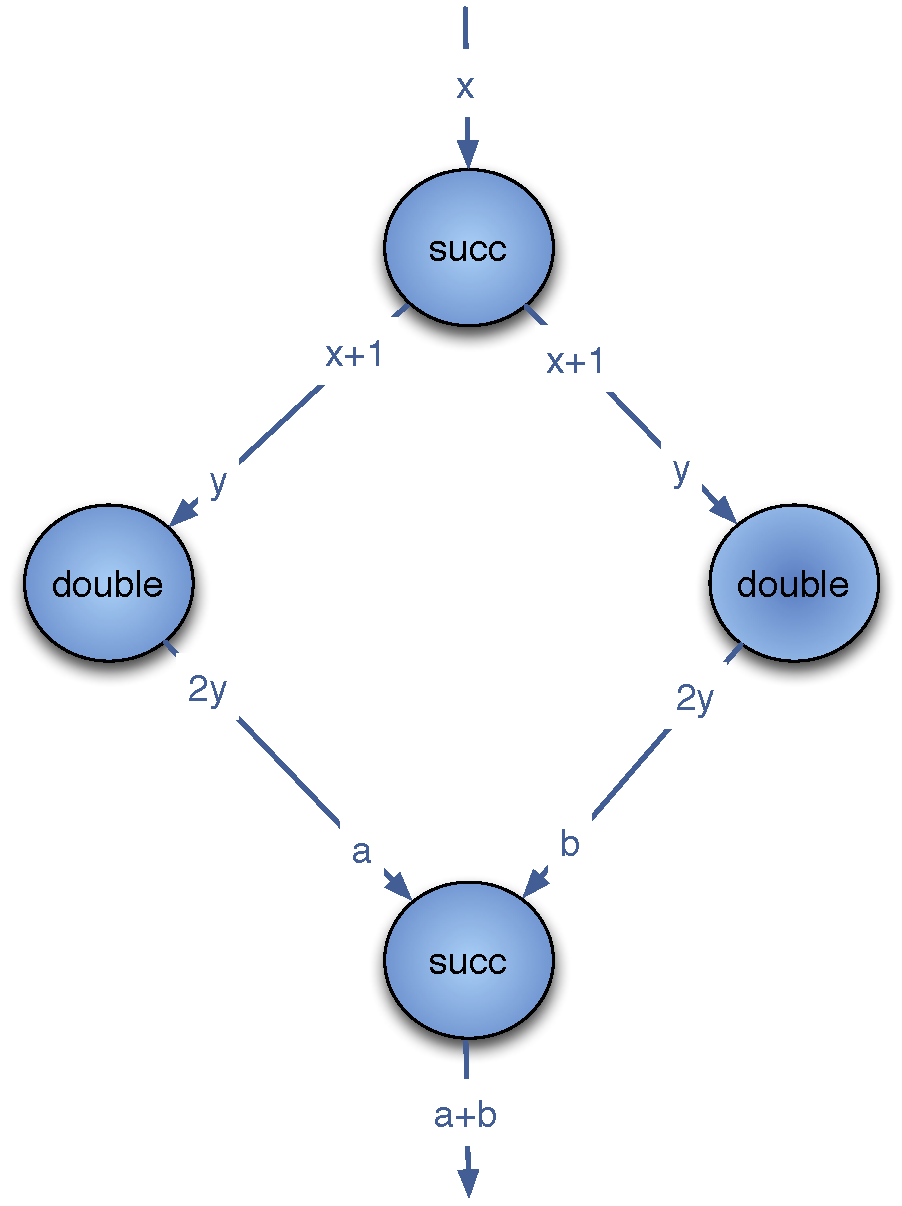
\includegraphics[keepaspectratio,width=0.4\linewidth]{fig/wf_example1}
  \caption{\DAG example}
  \label{fig:example1}
\end{figure}

\section{Software architecture}

A special agent, called a \textit{\madag}, is used to manage workflows in the
\diet architecture. It receives requests from clients containing the
description of a workflow in a specific language (the \madag XML workflow
language for \DAGS). The role of the \madag is to determine how to schedule the
tasks contained in the workflow in order to follow the precedence constraints
between tasks, and how to map the tasks to appropriate resources in the \diet
hierarchy.

The execution of individual tasks is actually delegated by the \madag to
the client that submitted the workflow. After submitting the workflow, the
client is put in a waiting mode and it will receive individual requests from
the \madag to execute each task of the workflow. Therefore all data
transfers are done only from the client to the {\sed}s and do not transit
through the \madag.

When all tasks are completed, the \madag sends a release signal to the
client which then retrieves the results if the execution was successful.

To use the \madag, the client configuration file must include the parameter
\texttt{MADAGNAME} with the appropriate name.

When the client uses a functional workflow (in Gwendia language) the \diet
client library provides the logic for instanciating the workflow, generating
the \DAGS and sending them to the \madag. Note that when several \DAGS are
generated, they are usually not independent as some data generated by one \DAG
may be used by another one.

\section{Workflow description languages}

\subsection{\madag language}
\label{sec:dag_desc}

A \DAG is described with an XML representation which is close to \diet profile
representation. In addition to the profile description (problem path and
arguments), this description represents also the data dependencies between
ports (source/sink), and contains the node identifiers (which must be unique in
the \DAG) and the precedences between nodes. This last information can be
partial since it can be retrieved from the dependencies between ports, however
it can be useful to define a temporal dependency without port linking (using
the {\texttt prec id} keyword, see {\texttt xml/matrix.xml} for such an
example).

The general structure of this description is:

\begin{verbatim}
<dag>
  <node id="..." path="...">
    <arg name="..." type="........" value=".."/>
    <in name="..." type="........" source="......."/>
    <out name="...." type="........" sink="......"/>
    <out name="...." type="........" sink="......"/>
  </node>
  ....
\end{verbatim}

A node is defined by its identity and the computing problem it requests, \ie
the problem {\it path}. For each node, an input data is either specified with a
line describing its name, type and possibly from which precedent node it has to
be transferred, either with a line describing its name, type and value in case
the data is not generated by a previous task. An output data is specified
within a line containing its name and type. Note the in order to use a data as
a \textit{source} or a \textit{sink}, {\it its name must be prefixed with the
  node identity} (which avoids name conflicts). 

For example the source of the input port \textit{in3} is the port \textit{out2}
of the node \textit{n1} and the data is a \verb! DIET_INT!, than the element
must be described as follow:

\begin{verbatim}
    <in name="in3" type="DIET_INT" source="n1#out2"/>
\end{verbatim}

The link between input and output ports must be described either by a
\textit{source} value in the \textit{$<$in$>$} element, or by a \textit{sink} value
in the \textit{$<$out$>$} element. Specifying both does not cause an error but
duplicates the information.

The example shown in Figure~\ref{fig:example1} can be represented by this XML
description:

\begin{verbatim}
<dag>
  <node id="n1" path="succ">
    <arg name="in1" type="DIET_INT" value="56"/>
    <out name="out1" type="DIET_INT"/>
    <out name="out2" type="DIET_INT"/>
  </node>
  <node id="n2" path="double">
    <in name="in2" type="DIET_INT" source="n1#out1"/>
    <out name="out3" type="DIET_INT"/>
  </node>
  <node id="n3" path="double">
    <in name="in3" type="DIET_INT" source="n1#out2"/>
    <out name="out4" type="DIET_INT"/>
  </node>
  <node id="n4" path="sum">
    <in name="in4" type="DIET_INT" source="n2#out3"/>
    <in name="in5" type="DIET_INT" source="n3#out4"/>
    <out name="out4" type="DIET_INT"/>
  </node>
</dag>
\end{verbatim}

\subsection{Gwendia language}
\label{sec:wf_desc}
The Gwendia language is written in XML and validated by the workflow parser if
the path to the DTD is provided (using a !DOCTYPE XML entity in the workflow
XML file). The Gwendia DTD is included in the \diet distribution in the
\verb|/usr/share/diet/FWorkflow.dtd| file.

\paragraph{Types} Values flowing through the workflow are typed.
Basic types are \texttt{integer}, \texttt{short}, \texttt{double},
\texttt{longint}, \texttt{float}, \texttt{string} and
\texttt{file}. Homogeneous arrays of values can be also used as inputs/outputs
and can have any \textit{depth}: an array can contain arrays of values (depth =
2). Arrays are ordered and can eventually contain \textit{NULL} elements.

\paragraph{Processors} A \texttt{processor} is a data production unit. 
A regular processor invokes a service through a known interface. Defined
processor types are \texttt{webservice}, \texttt{diet} and
\texttt{beanshell}. Special processors are workflow \texttt{source} (a
processor with no inbound connectivity, delivering a list of externally defined
data values), \texttt{sink} (a processor with no outbound connectivity,
receiving some workflow output) and \texttt{constant} (a processor delivering a
single, constant value). To improve readability, the \texttt{source},
\texttt{sink} and \texttt{constant} processors are grouped in an
\texttt{<interface>} tag within the document. Other example of processors are
grouped in a \texttt{<processors>} tag. Web services define a \texttt{<wsdl>}
tag pointing to their WSDL description and the operation to invoke. Beanshells
define a \texttt{<script>} tag containing the java code to interpret. \diet
services define a \texttt{<diet>} tag describing the path to service to
invoke. (When executing the workflow using the \diet workflow engine, only
processors containing a \texttt{<diet>} tag can be used). The \texttt{<diet>}
tag contains the \texttt{path} attribute that matches exactly the \diet service
name, and optionnally contains the 'estimation' attribute (with value keyword
'constant') whenever the computation time estimation for this service does not
depend on input data (using this option may reduce considerably the load on the
\diet platform because the request for performance estimation is done only once
by the \madag instead of being done for each task).

\paragraph{Processor ports} 
Processor input and output ports are named and declared. A port may be an input
(\texttt{<in>} tag) or an output (\texttt{<out>} tag). For each input/output, the
following attributes can be defined:
\begin{itemize}
\item \texttt{type} (mandatory): contains the base type of data \ie a basic
type identifier that describes the type of the data received/generated by the
  port. When data is scalar this is the actual data type, when data is an array
  this is the type of the data leaves of the array.
\item \texttt{depth} (optional, default is 0): contains the depth of the array
  if applicable
\item \texttt{cardinality} (optional, only for out ports with depth $>0$):
  contains the number of elements of the generated array. This value can be
  provided only if it is a constant \ie the number of elements does not vary
  for each instance of data. When the data depth is greater than 1, the format
  for the cardinality attribute is a column-separated list of integers (for
  example, "2:3" for an array containing 2 arrays of 3 elements).
\end{itemize}

\paragraph{Iteration strategies} 
Iteration strategies must be defined when the processor has two or more input
ports. By default the workflow parser will use a \textit{dot} iteration
strategy for all inputs. These operators use the \texttt{index} of data items
received or produced by workflow processors to combine them. The index of a
data item corresponds, for data items produced by a \texttt{source} to the
order number in the source data file, and for data items produced by a standard
processor to the index of input data items eventually combined by the
operators.  There are 4 data manipulation operators:
\begin{itemize}
\item \texttt{dot} (groups 2 or more ports): data from the different
  ports are processed together when their index match exactly (data
  with index 0 of one port is matched with data with index 0 of the
  other ports). The output index is the same as the index of the input
  data.
\item \texttt{cross} (groups 2 ports): processes each data instance of
  the first port with each data instance of the second port. This
  processor will increase by one the index depth of the output (for
  example: if data inputs have indexes 0 and 1 then the outputs have
  the index 0\_1).
\item \texttt{flatcross} (groups 2 ports): same as cross but with a
  different output indexation scheme. This operator does not increase
  the depth of the output index but creates new indexes (\eg
  if data inputs have indexes 1 and 2 with a maximum index of 3 for
  the right input, then the output has the index $6 = 4*1 + 2$). Note
  that this operator creates a synchronization constraint among all
  instances as the maximum index of the right input must be known by
  the workflow engine before being able to create new indexes.
\item \texttt{match} (groups 2 ports): processes each data instance of
  the first port with all the data instances of the second port that
  have an index prefix that matches the first port's index (for
  example: if left data has index 1\_1, it will be processed with all
  right data which have an index beginning with 1\_1). The output
  index is the second port's index.
\end{itemize}

\fixme{Add figures explaining the different iteration strategies}

Here is an example of a Gwendia workflow (to be continued with the links part
below):

\begin{verbatim}
<workflow>
  <interface>
    <constant name="parameter" type="integer" value="50"/>
    <source name="key" type="double" />
    <sink name="results" type="file" />
  </interface>

  </processors>
    <processor name="genParam">
      <in name="paramKey" type="double"/>
      <out name="paramFiles" type="file" depth="1"/>
      <diet path="gen" estimation="constant"/>
    </processor>

    <processor name="docking">
      <in name="param" type="integer" />
      <in name="input" type="file" />
      <out name="result" type="double" />
      <iterationstrategy>
        <cross>
          <port name="param" />
          <port name="input" />
        </cross>
      </iterationstrategy>
      <diet path="dock" estimation="constant"/>
    </processor>

    <processor name="statisticaltest">
      <in name="values" type="double" depth="1"/>
      <out name="result" type="file"/>
      <iterationstrategy>
        <cross>
          <port name="coefficient" />
          <match>
            <port name="values" />
            <port name="weights" />
          </match>
        </cross>
      </iterationstrategy>
      <diet path="weightedaverage" />
    </processor>
</processors>
<links>
  <!-- LINKS (see below) -->
</links>
</workflow>
\end{verbatim}

\paragraph{Data links} A data link is a connection between a processor output port and a processor input port as exampled below:
\begin{verbatim}
<links>
    <link from="key" to="genParam:paramKey"/>
    <link from="genParam:paramFiles" to="docking:input"/>
    <link from="parameter" to="docking:param"/>
    <link from="docking:result" to="statisticaltest:values" />
    <link from="statisticaltest:result" to="results" />
</links>
\end{verbatim}
When a processor A (port A.out) is connected to a processor B (port B.in)
through a data link, an instance of A (one task) may trigger a number of B
instances that depends on first, the data depth at both ends of the link and
second, the iteration strategy chosen for the B.in port within the B processor.


The data depths on both ends of the link determine the number of data
items received by the B.in port. Three cases are possible:
 \begin{itemize}
\item \texttt{1 to 1} : when depth(A.out) $=$ depth(B.in), a data item produced
  by A.out is sent as-is to B.in
\item \texttt{1 to N} : when depth(A.out) $<$ depth(B.in), a data item produced
  by A.out is an array that will be split into its elements when sent to
  B. This will produce several parallel instances (tasks) of the B
  processor. This is equivalent to a \textit{foreach} structure in usual
  programming languages, but is here transparent for the user as this is the
  workflow engines that manages it.
\item \texttt{N to 1} : when depth(A.out) $>$ depth(B.in), several data items
  produced by A.out (by \textit{different} tasks) will be grouped in an array
  before being sent to B.in. This is the opposite behaviour from the previous
  point. Note that this structure creates a synchronization barrier among the A
  tasks as they must all be completed before the B tasks can be launched.
 \end{itemize}

\paragraph{Conditionals (if/then/else)} Specific out ports tags (\texttt{<outThen>} and \texttt{<outElse>}) are
used in that kind of node. An outThen port will receive data assigned according
to the assignment list in the \texttt{<then>} tag only when the condition is
evaluated to true. If the condition is false, this port will not receive data
but the \texttt{<outElse>} port will receive data according to the assignment
list in the \texttt{<else>} tag (assignment lists are semi-column separated
lists of assignments of an outThen or outElse port to an input port).
\begin{verbatim}
  <condition name="IF_Example">
    <in name="i" type="integer" />
    <in name="j" type="integer" />
    <outThen name="out1" type="integer" />
    <outElse name="out2" type="integer" />
    <!-- IF Condition must be written in XQuery language -->
    <if>$i lt $j</if>
    <then>out1=i;</then>
    <else>out2=j;</else>
  </condition>
\end{verbatim}
Note that all the operators and functions defined in the XQuery standard (see
\url{http://www.w3.org/TR/xquery-operators/}) can be used to make the boolean
expression of the \texttt{<if>} tag. These can process both numerical and
string variables, and can also contain XPath expressions to access elements of
an array when the input port type is an array (\eg the expression ``
\texttt{contains(\$in\/list\/item[1]\/text(), 'a')} '' tests if the 1st element
of the array provided by the 'in' port contains the letter 'a').


\paragraph{While loops}  
This structure uses specific port tags (\texttt{<inLoop>} and
\texttt{<outLoop>}) in addition to standard port tags. They are used to connect
this processor to other processors that will be iterated as long as the while
condition is true (condition is evaluated \textit{before} the first
iteration). The standard \texttt{<in>} and \texttt{<out>} ports are used to
connect this processor to the rest of the workflow.

The loop initialization is done by mapping data from in ports to inLoop ports
using the 'init' attribute. Each iteration produces data on outLoop ports
according to the assignments of the \texttt{<do>} tag (semi-column separated
list of assignments). The outputs of the processors that are iterated can be
connected to the inLoop ports when the results of one iteration are used by the
next one (but this is not mandatory). When the while condition is evaluated to
false, the outLoop data items are handed over to the corresponding out ports
according to the 'final' attribute of these. They are then sent to the
connected processors.

Finally for one instance of this \textit{while} processor, $N \geq 0$
iterations are done for processors connected to the outLoop ports and one data
item is produced by the out port(s).

\begin{verbatim}
  <loop name="WHILE_Example">
    <!-- REQUIRED nb of IN ports EQUALS nb of OUT ports -->
    <in name="v" type="double" />
    <out name="out" type="double" />

    <inLoop name="v_l" type="double" init="v"/>
    <outLoop name="l" type="double" final="out"/>

    <!-- WHILE Condition must be written in XQuery language -->
    <!-- it can contain ONLY LOOP IN ports -->
    <while>$v lt 100</while>

    <!-- DO maps the inLoop ports to the outLoop ports - straightforward -->
    <do>l=v_l;</do>

  </loop>
\end{verbatim}

\section{Client API}

\subsection{Structure of client program}
\label{sec:client_prg}

The structure of a client program is very close to the structure of usual \diet
client. The general algorithm is as follow:

\begin{verbatim}
diet_initialize

create the workflow profile

call the method diet_wf_call

if success retrieve the results

free the workflow profile

diet_finalize
\end{verbatim}

The following tables show a description of methods provided by the \diet
workflow API. The table~\ref{tab::wf_common_api} contains the main methods that
are common to the \DAG workflows API and to the functional workflows API.  The
table~\ref{tab::wf_dag_api} contains the methods that are specific to the \DAG
API. The table~\ref{tab::wf_gw_api} contains the methods that are specific to
the functional workflows API.

\begin{table}[htbp]
  \centering
  \begin{tabular}[htbp]{|p{8cm}|p{7.5cm}|}\hline
    Workflow function & Description \\\hline
    %
    \texttt{diet\_wf\_desc\_t*  \newline
      diet\_wf\_profile\_alloc(const char* wf\_file\_name, const char* wf\_name, wf\_level\_t wf\_level);}
    &
    allocate a workflow profile to be used for a workflow submission.\newline
    \textit{wf\_file\_name} : the file name containing the workflow XML description.
    \textit{wf\_name} : the name of the workflow (used for logs)
    \textit{wf\_level} : specifier for workflow type (\DAG or FUNCTIONAL)
    \\\hline

    %
    \texttt{void  \newline
      diet\_wf\_profile\_free(diet\_wf\_desc\_t * profile);}
    &
    free the workflow profile.
    \\\hline
    %
    \texttt{diet\_error\_t \newline
      diet\_wf\_call(diet\_wf\_desc\_t* wf\_profile);}
    &
    execute the workflow associated to profile \textit{wf\_profile}.
    \\\hline
    %
    \texttt{int \newline
      diet\_wf\_print\_results(diet\_wf\_desc\_t * profile);}
    &
    print on standard output all the results of the current executed workflow or \DAG.
    \\\hline
    %
  \end{tabular}
  \caption{\diet workflow common API}
  \label{tab::wf_common_api}
\end{table}

\begin{table}[htbp]
  \centering
  \begin{tabular}[htbp]{|p{8cm}|p{7.5cm}|}\hline
    Workflow function & Description \\\hline
    %
    \texttt{int   \newline
      diet\_wf\_scalar\_get(const char * id, void** value);}
    &
    retrieves a workflow scalar result. \newline
    \textit{id} : the output port identifier.
    \\\hline
    %
    \texttt{int   \newline
      diet\_wf\_string\_get(const char * id, char** value);}
    &
    retrieves a workflow string result. \newline
    \textit{id} : the output port identifier.
    \\\hline
    %
    \texttt{int    \newline
      diet\_wf\_file\_get(const char * id, size\_t* size, char** path);}
    &
    retrieves a workflow file result. \newline
    \textit{id} : the output port identifier.
    \\\hline
    %
    \texttt{int    \newline
      diet\_wf\_matrix\_get(id, (void**)value, nb\_rows, nb\_cols, order);}
    &
    retrieves a workflow matrix result. \newline
    \textit{id} : the output port identifier.
    \\\hline
    %
  \end{tabular}
  \caption{\diet workflow \DAG-specific API}
  \label{tab::wf_dag_api}
\end{table}

\begin{table}[htbp]
  \centering
   \begin{tabular}[htbp]{|p{8cm}|p{7.5cm}|}\hline
    Workflow function & Description \\\hline
    %
    \texttt{void  \newline
      diet\_wf\_set\_data\_file( \newline
        diet\_wf\_desc\_t * profile, \newline
        const char * data\_file\_name);}
    &
    specifies the file containing the data description used to generate the workflow
    \\\hline
    %
    \texttt{void  \newline
      diet\_wf\_set\_transcript\_file(  \newline
        diet\_wf\_desc\_t * profile,  \newline
        const char * transcript\_file\_name);}
    &
    specifies the file containing the tasks status and data (used to restart a \DAG or workflow)
    \\\hline
    %
    \texttt{int \newline
      diet\_wf\_save\_data\_file(  \newline
        diet\_wf\_desc\_t * profile,  \newline
        const char * data\_file\_name);}
    &
    saves the input and output data description ('source' and 'sink' nodes) in XML format.
    The file can be used as input data file for another workflow execution.
    \\\hline
    %
    \texttt{int \newline
      diet\_wf\_save\_transcript\_file( \newline
        diet\_wf\_desc\_t * profile,  \newline
        const char * transcript\_file\_name);}
    &
    saves the transcript of the current workflow (list of tasks with their status and data).
    This file can be used as input transcript file for another workflow execution (tasks already done
    with output data still available on the platform will not be executed again)
    \\\hline
    %
    \texttt{int \newline
      diet\_wf\_sink\_get(  \newline
        diet\_wf\_desc\_t* wf\_profile, \newline
        const char * id, char** dataID;}
    &
    gets a container (\dagda data) containing all the data received by a 'sink' node
    \\\hline
    %
    \end{tabular}
    \caption{\diet workflow Functional-specific API}
\label{tab::wf_gw_api}
\end{table}


%\subsection{Examples}
\subsection{The simplest example}
\label{sec:examples}

%\subsubsection{The simplest example}
\label{sec:ex1}

This example represents the basic client code to execute a \DAG. Line 26
indicates that the workflow output is a double value named \verb|n4#out4|. The
example shown in Figure~\ref{fig:example1} can be fully (execution and result
retrieving) executed with this client.

\begin{lstlisting}{1}
#include <string.h>
#include <unistd.h>
#include <stdlib.h>
#include <stdio.h>
#include <sys/stat.h>

#include "DIET_client.h"

int main(int argc, char* argv[])
{
  diet_wf_desc_t * profile;
  char * fileName;
  long * l;
  if (argc != 3) {
    fprintf(stderr, "Usage: %s <file.cfg> <wf_file> \n", argv[0]);
    return 1;
  }

  if (diet_initialize(argv[1], argc, argv)) {
    fprintf(stderr, "DIET initialization failed !\n");
    return 1;
  }
  fileName = argv[2];
  profile = diet_wf_profile_alloc(fileName,"test",DIET_WF_DAG);
  if (!diet_wf_call(profile)) {
    printf("get result = %d ", diet_wf_scalar_get("n4#out4", &l));
    printf("%ld\n", (long)(*l));
  }
  diet_wf_free(profile);
  return 0;
}
\end{lstlisting}

\section{Scheduling}
\label{sec:wf_sched}

The \madag agent may receive many requests to execute workflows from one or
several clients, and the number of ressources to execute all tasks in parallel
may not be sufficient on the grid. In this case the choice of a particular
workflow scheduler is critical to determine the order of execution of all tasks
that are ready to be executed.

Schedulers provide different online scheduling heuristics that apply different
prioritization algorithms to choose the order of execution between tasks of the
same \DAG (intra-\DAG priority) and between tasks of different \DAGS (inter-\DAG
priority). All heuristics are based on the well-known HEFT heuristic that is
extended to this case of online multi-workflow scheduling.

\subsection{Available schedulers}

The available \madag workflow schedulers are:

\begin{itemize}

\item A basic scheduler (option -basic or default choice): this scheduler
  manages the precedence constraints between the tasks. The priority between
  tasks within a \DAG is set according (Heterogeneous Earliest Finish Time)
  HEFT~\cite{heft_cpop} heuristic. When a task is ready to be executed (\ie the
  preceding tasks are completed) the ready task with the higher HEFT rank is
  sent to the client for execution without specifying a ressource. Then the
  client performs a standard \diet request that will use the scheduler
  configured by the \sed.

\item A Multi-HEFT scheduler (option -heft): this scheduler applies the HEFT
  heuristic to all workflows submitted by different clients to the \madag. This
  means that the priorities assigned by the HEFT heuristic are used to order
  the tasks of all \DAGS processed by the \madag and following this order the
  tasks are mapped to the first available ressource.

\item A Multi-AgingHEFT scheduler (option -aging\_heft): this scheduler is
  similar to Multi-HEFT but it applies a correction factor to the priorities
  calculated by the HEFT algorithm. This factor is based on the age of the \DAG
  ie the time since it was submitted to the scheduler. Compared to Multi-HEFT
  this scheduler will increase the priority of the tasks of a workflow that has
  been submitted earlier than other \DAGS.

\item A FOFT (Fairness on Finish Time) scheduler (option -fairness): this
  scheduler uses another heuristic to apply a correction factor to the
  priorities calculated by the HEFT algorithm. This factor is based on the
  slowdown of the \DAG that is calculated by comparing the earliest finish time
  of the tasks in the same environment without any other concurrent workflow
  and the actual estimated finish time.

\end{itemize}

\subsection{\sed requirements for workflow scheduling}

The workflow schedulers (Basic, Multi-HEFT, Multi-AgingHEFT and FOFT) use
information provided by the {\sed}s to be able to run the HEFT heuristic. So
the \sed programmer must provide the required data in the estimation vector by
implementing a plugin scheduler (see chapter~\ref{ch:plugin}).

The following fields in the estimation vector must be filled in:
\begin{enumerate}
\item The \texttt{TCOMP} field must contain the estimation of the computation
  time for the job (in milliseconds). This can be done using the
  \texttt{diet\_estimate\_comptime(estVector\_t ev, double value)} method
  within the performance evaluation function.
\item The \texttt{EFT} field must contain the estimation of the earliest finish
  time (in milliseconds from the time of the current submit request) for the
  job. To compute this value, the \sed programmer can use the API method
  \\ \texttt{diet\_estimate\_eft(...)} to retrieve the estimated value of
  earliest finish time for a new job.
\end{enumerate}

% \subsection{Writing a new scheduler}
%
% The workflow scheduler of the client is different little bit from the
% MA\_DAG one. To write a new scheduler you need diet sources. The
% following two section show how to develop your own scheduler and how
% to plug it in your client or in the MA\_DAG.
%
% \paragraph{Client scheduler}
%
% To write a new workflow scheduler for your diet client you need to
% create a derived class of the base abstract class
% \textit{AbstractWfSched}. The main function of the scheduler (the SeDs
% mapping) must be placed in the pure virtual function \textit{execute}.
% These are the steps to follow:
%
% \begin{enumerate}
% \item Write a subclass of \textit{AbsWfSched} abstract class. The
%   virtual method \textit{execute} needs to be implemented.
% \item Create a c++ file where you can put the following code:
% \begin{verbatim}
% extern "C" {
%   void set_my_personal_sched() {
%     Personal_WfSched * mySched = new Personal_WfSched();
%     set_sched(mySched);
%   }
% }
% \end{verbatim}
% \item In your client source code, call the method
%   \textit{set\_my\_personal\_sched} before executing the
%   \textit{diet\_wf\_call}.
% \item Link the previous c++ object code to you \diet client.
% \end{enumerate}

%%% Local Variables:
%%% mode: latex
%%% ispell-local-dictionary: "american"
%%% mode: flyspell
%%% fill-column: 79
%%% End:
